\section{Quantum Picturalism}
\label{sec:QP}

Quantum Picturalism (QP) is an innovative approach to studying, teaching and practising quantum theory, relying on diagrammatic languages to conceptualise and manipulate highly abstract mathematical notions.

Its roots can be traced back to work by Penrose in the early 1970s, introducing early examples of graphical notation for tensors~\cite{Penrose}.
Work by Joyal and Street in the 1990s~\cite{JS} freed such graphical notations from the shackles of the physics that birthed them, introducing string diagrams as a language for a much broader realm of pure and applied mathematics within the unifying framework of category theory.
A specialisation of string diagrams to the algebraic structures of quantum theory in the early 2000s finally resulted in categorical quantum mechanics~\cite{abramsky2004categorical,coecke2006kindergarten,abramsky2009categorical}, the mathematical foundation for the QP approach.

QP is a multi-faceted framework with a variety of diagrammatic languages that capture quantum phenomena from different perspectives.
Of these languages, one of the oldest and most widely adopted is the ZX-calculus~\cite{coecke2011interacting}. Since its inception 12 years ago, the ZX-calculus has quickly found applications in quantum circuit optimisation~\cite{duncan2020graph, de2020fast, de2019techniques, kissinger2019reducing}, quantum error correction~\cite{huang2023qeczx, de2020zx, kissinger2022phase, khesinGraphicalQuantumCliffordencoder2023}, quantum simulation~\cite{kissinger2022classical}, quantum foundations~\cite{coecke2011phase, backens2016complete, gogioso2019dynamics, gogioso2017mermin}, measurement-based quantum computing~\cite{coecke2008interacting, duncan2009graph, kissinger2019universal}, quantum natural language processing~\cite{QPL-QNLP, lorenz2021qnlp, coecke2020foundations} and more. For learning resources on the ZX-calculus, adequate for all levels of familiarity with quantum theory, we refer to the ``Getting started'' section of \href{https://zxcalculus.com/#introPublications}{zxcalculus.com}.

Analogous diagrammatic approaches based on string diagrams have established themselves in several other scientific fields, including computer science~\cite{bonchi2014categorical}, linguistics~\cite{sadrzadeh2013frobenius, wang2023distilling}, and causal reasoning~\cite{lorenz2023causal}.
Several valuable variants of the ZX-calculus are used for quantum applications, such as the ZH-calculus~\cite{backens2018zh}, to study traditional quantum algorithms based on the quantisation of classical computation; and the ZXW-calculus~\cite{poor2023completeness}, with applications from photonic quantum computing~\cite{defelicelightmatterZXW} to Hamiltonian simulations and quantum chemistry~\cite{shaikh2022sum}.

The content and presentation for the course are based on the recently published book ``Quantum in Pictures''~\cite{coecke2022quantum}, by Coecke and Gogioso.
The book is an accessible version of the university-level textbook ``Picturing Quantum Processes: A First Course on Quantum Theory and Diagrammatic Reasoning''~\cite{CKbook}, by Coecke and Kissinger.
Material from ``Picturing Quantum Processes'' has been used for almost a decade at the University of Oxford for several courses in quantum theory offered by the Department of Computer Science.
In addition to being more accessible, engaging and reader-friendly, ``Quantum in Pictures'' is up-to-date with cutting-edge research, including content that did not even exist when ``Picturing Quantum Processes'' was published in 2017.

As an example to explain the differences between QP and traditional approaches to quantum theory, we now turn our attention to the quantum teleportation protocol.
Quantum teleportation is a peculiar effect---of interest in both quantum foundations and measurement-based quantum computing---where the state of a quantum system is transferred across arbitrary distances by encoding it into a string of classical bits.
The advantage of doing this lies in the observation that quantum systems are fragile and highly sensitive to noise, while classical bits can be stored, replicated, manipulated and transferred with ease.

\begin{figure*}[h]
\centering
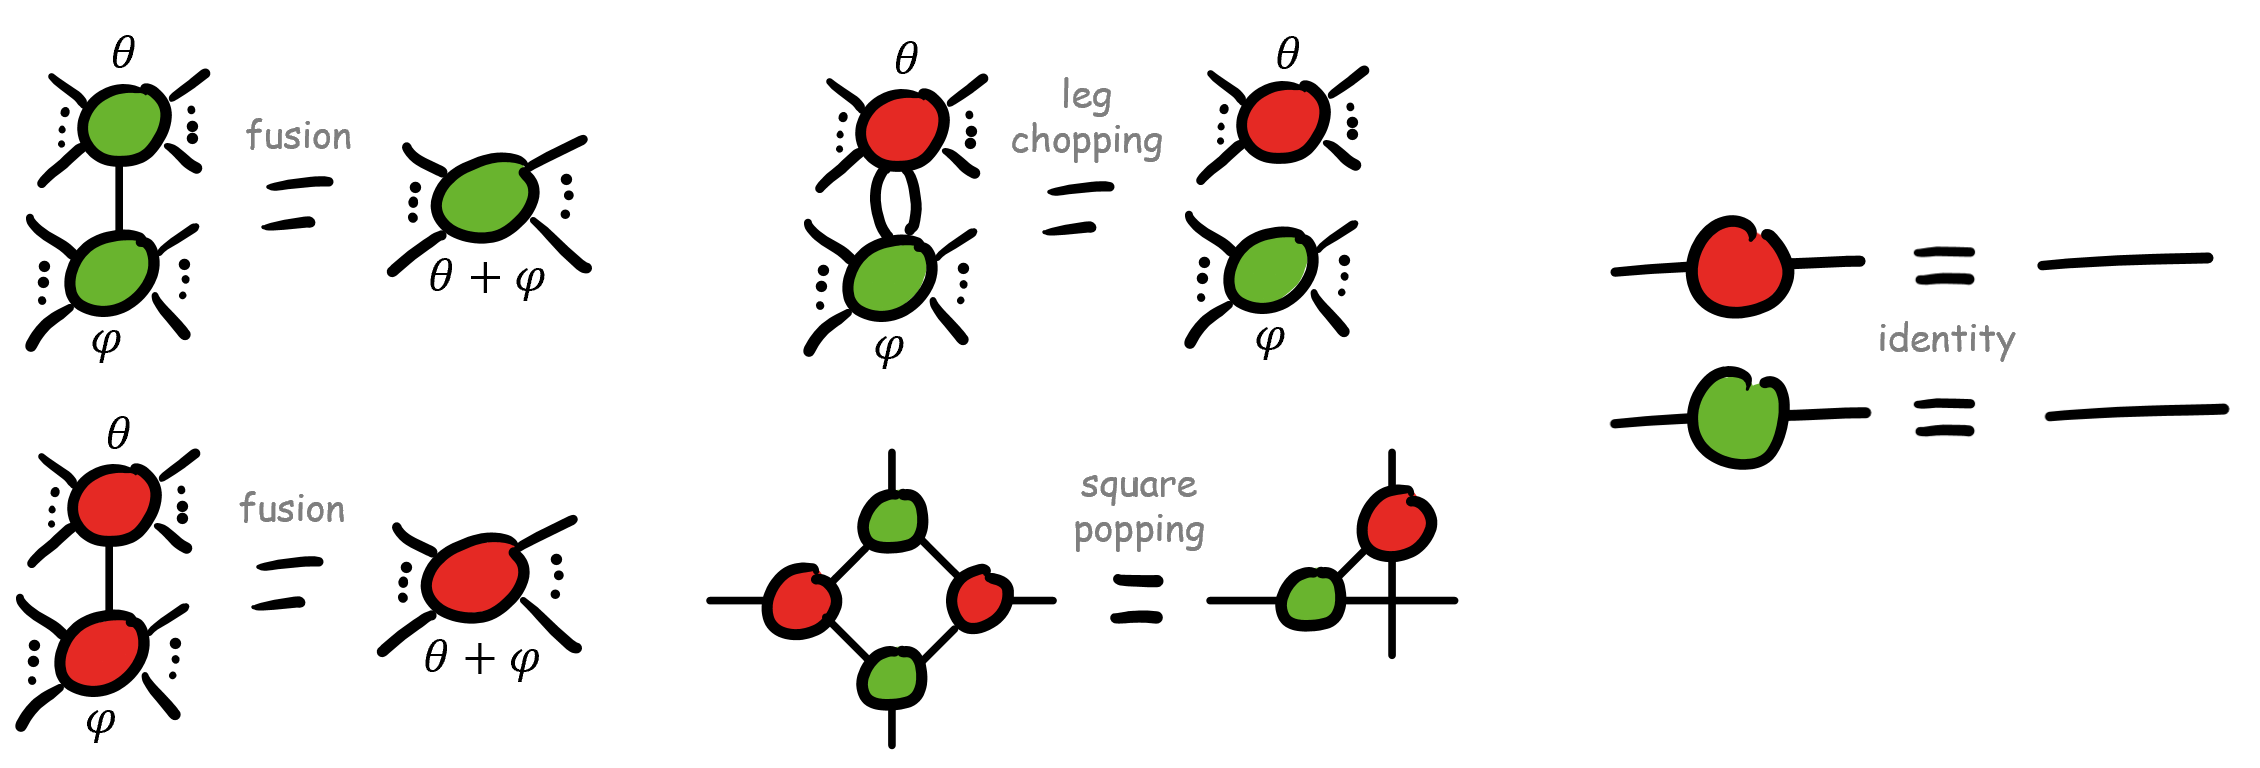
\includegraphics[width=0.8\textwidth]{Sections/pictures/zx-rules.png}
\caption{A selection of diagrammatic substitution rules for the ZX calculus, the visual language used by the Quantum Picturalism approach to Quantum Theory.}
\label{fig:zx-rules}
\end{figure*}

Figure \ref{fig:teleportation-learning} above exemplifies how quantum teleportation is introduced in a typical quantum information course.
It showcases two salient features of the traditional Hilbert space approach: (1) the heavy reliance on symbolic algebra---typically, Dirac's bra-ket notation---for the explicit description of quantum systems and calculations associated with their transformations; and (2) the need to employ a separate graphical notation---typically, quantum circuit notation---to explain the spatiotemporal layout of said quantum system and keep track of the operations acting upon them.
The shortcoming of the often-used combination of bra-ket notation and quantum circuit notation, is that the quantum circuit notation shows the operations of the protocol whereas the bra-ket computation shows the final result, but there is missing a representation of the intermediate steps bridging the two notations. In contrast, the QP proof makes clear the role of the Bell state and Bell measurement: The colors indicate that the CNOT gate, the $|0\rangle$ state, and the $|+\rangle$ state exhibit interaction of the Z (green) and X (red) observables, a fundamental observation that is not made evident by the quantum circuit, bra-ket, or matrix formalism. This corroborates previous observation that students in physics ``have difficulties with representations of quantum operators corresponding to observables especially when using Dirac notation''~\cite{Marshman2016difficultqoperators}. In a sense, the QP formalism makes it immediately clear that various components of quantum circuits are made ``of the same stuff'', and therefore interact in interesting ways (hence the title of the first ZX-calculus paper, `Interacting Quantum Observables'~\cite{coecke2011interacting}).

Below is the QP description of the quantum teleportation protocol, written in the diagrammatic language of the ZX-calculus.
Only two diagrammatic ingredients are needed: red and green circles---known as ``spiders''---annotated by angles and connected by lines.
The angles---known as ``phases''---indicate the extent to which qubits are rotated by various parts of the protocol, while the lines---known as ``wires''---indicate the exchange of quantum information (physical or virtual).
\begin{center}
    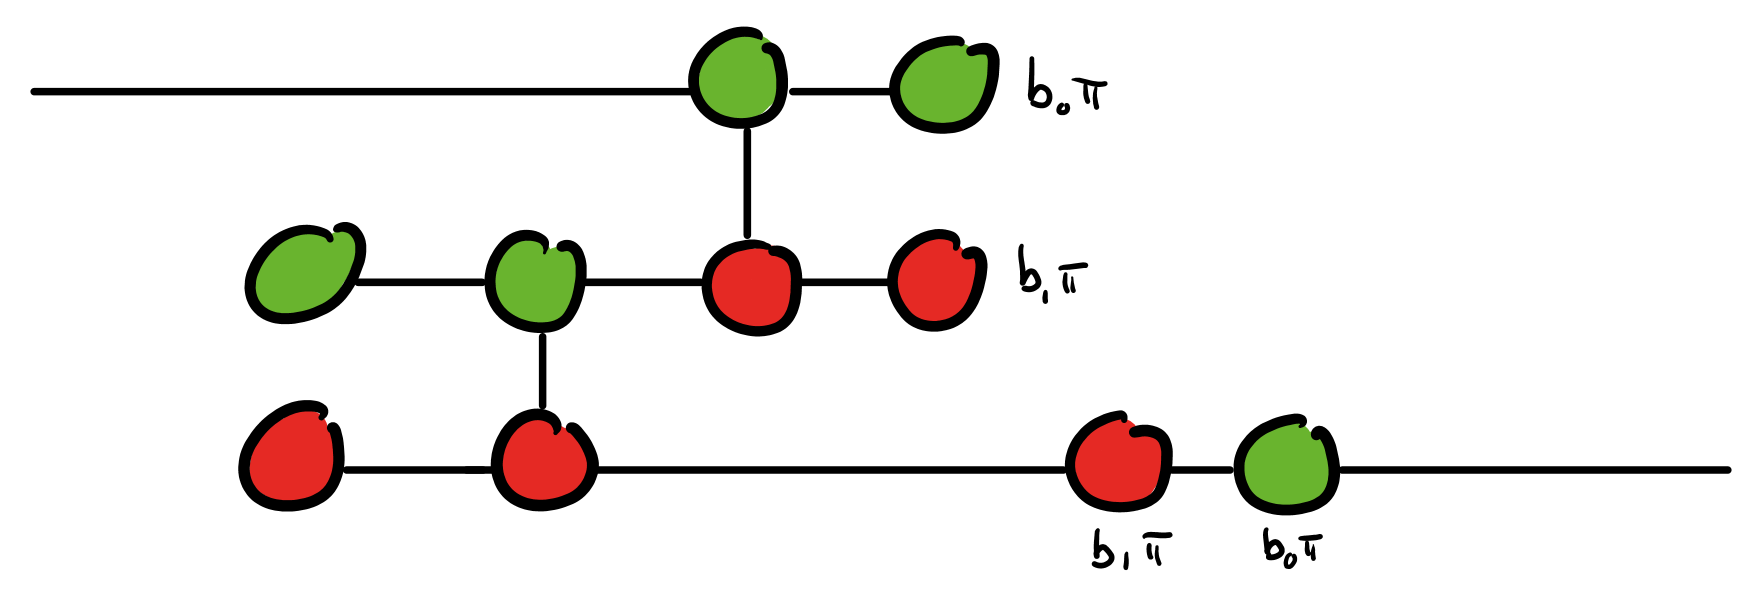
\includegraphics[width=0.4\textwidth]{Sections/pictures/teleportation-zx-raw.png}
\end{center}
Below is an annotated version of the same figure, indicating which parts of the ZX-diagram correspond to which parts of the traditional quantum circuit representation: the protocol takes a qubit as input (the wire on the left), results in a qubit as output (the wire on the right), and it involves two additional qubits, prepared in specified initial states (on the bottom left).
Two CNOT gates are applied to the three qubits, two of which are then measured (on the top right). A CNOT gate is a pair of a green spider and a red spider, connected by a vertical wire, with two wires on the left indicating the input qubits and two wires on the right indicating the output qubits.
The measurement outcomes, the bits $b_0$ and $b_1$, are then used to perform ``corrections'' on the remaining qubit in the form of two rotations (on the bottom right).
\begin{center}
    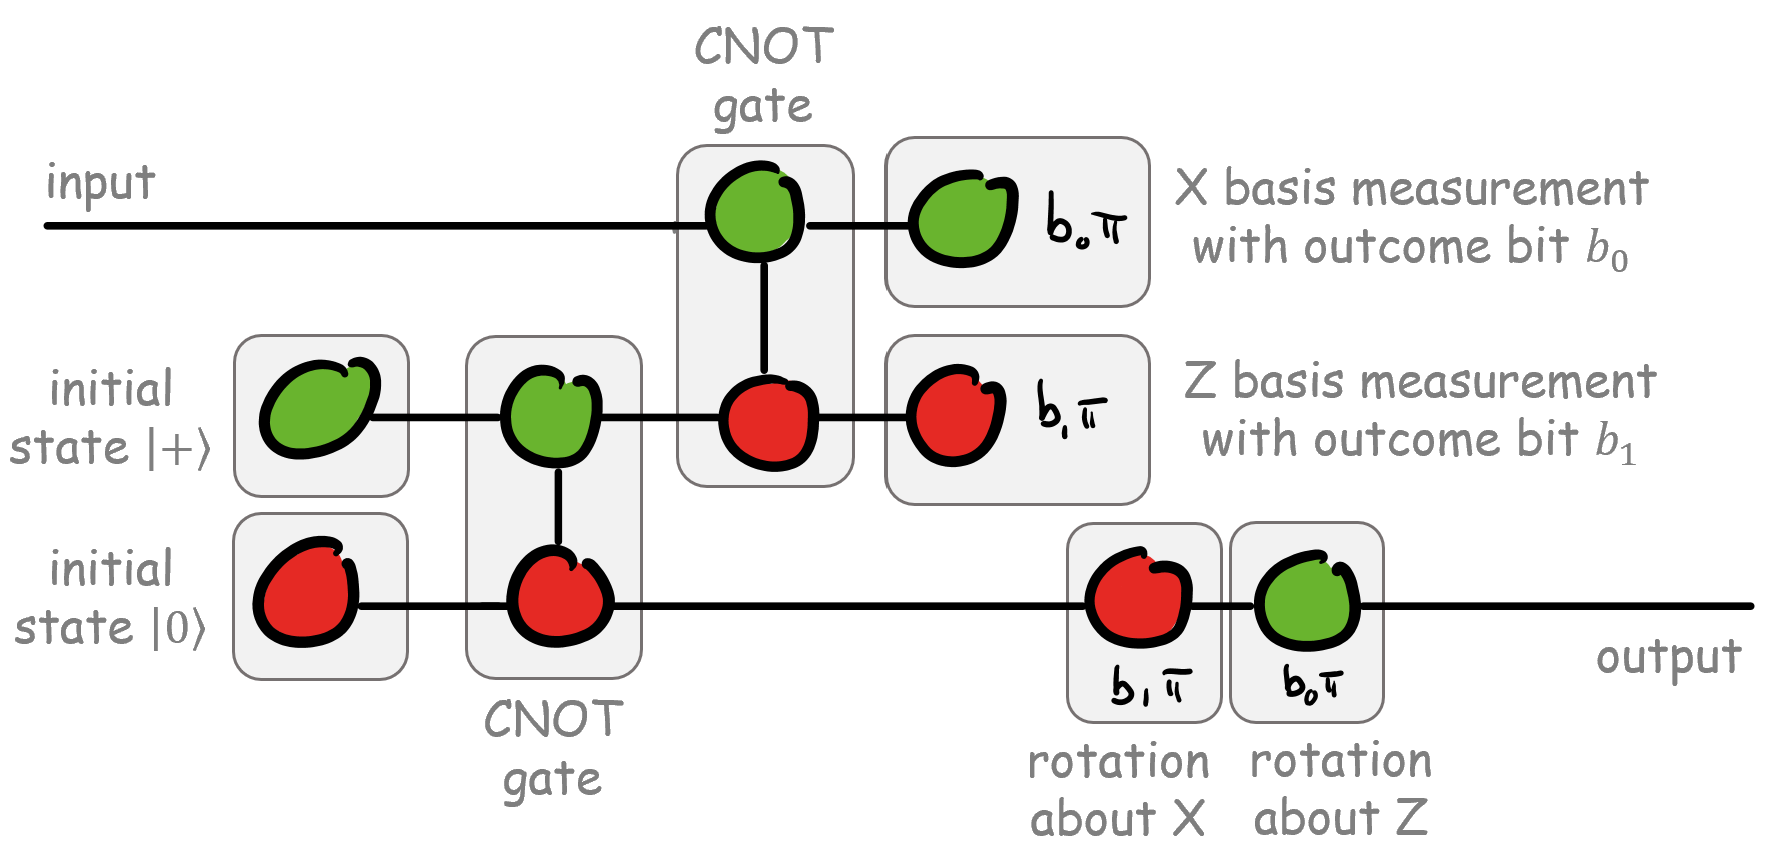
\includegraphics[width=0.45\textwidth]{Sections/pictures/teleportation-zx-annotated.png}
\end{center}
Without knowing much about the ZX-calculus, a comparison with Fig. \ref{fig:teleportation-learning} already highlights one of the critical features of QP: It reveals that parts which appear very different in the quantum circuit representation---initial states, CNOT gates and measurements---are composed of the same basic building blocks---red and green spiders---wired together in different patterns.

\begin{figure*}
\centering
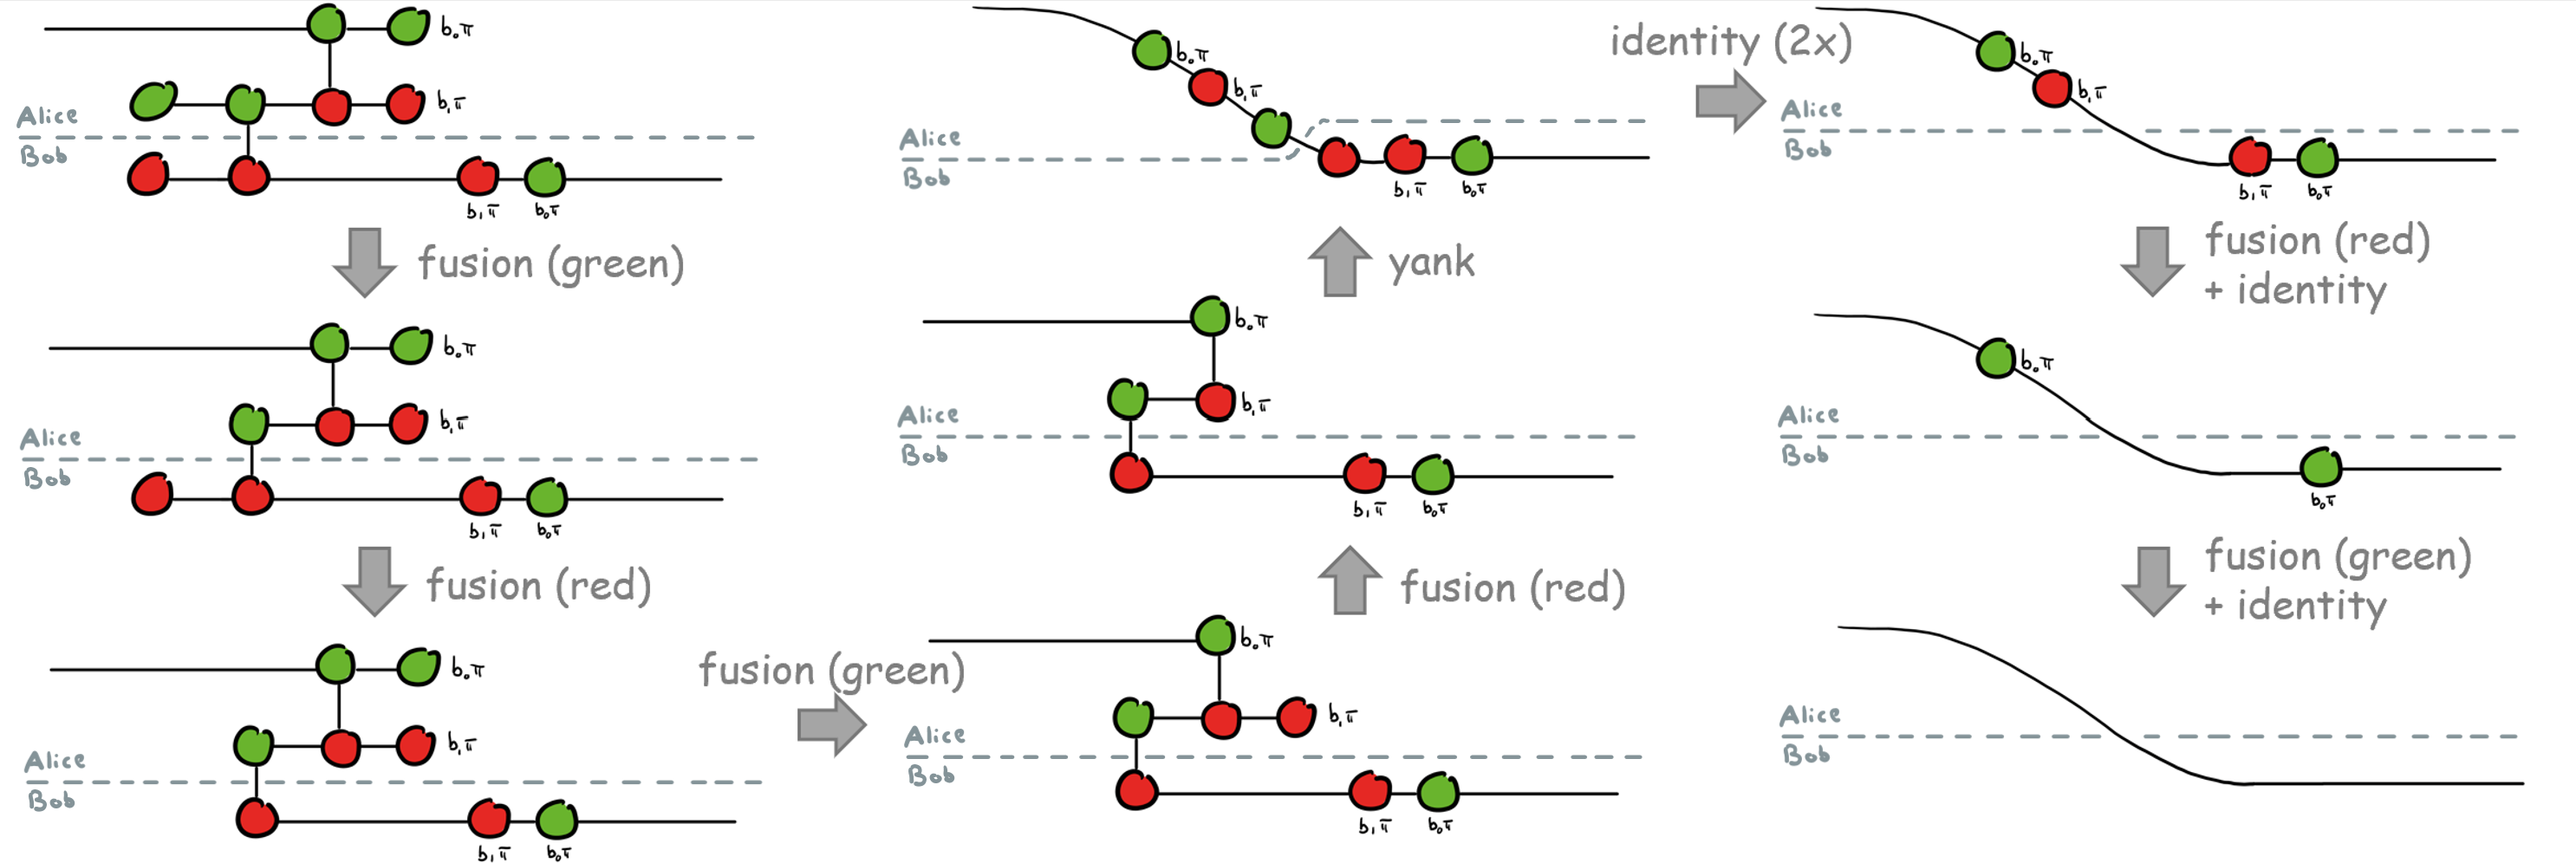
\includegraphics[width=\textwidth]{Sections/pictures/diagrammatic-reasoning-teleportation-steps-with-lines.png}
\caption{
Proof of correctness for the quantum teleportation protocol. This is the QP analogue of the Hilbert space calculations from Fig. \ref{fig:teleportation-learning} (p.\pageref{fig:teleportation-learning}). Each step of the proof is labeled with the diagrammatic rule of the ZX-calculus in Fig.~\ref{fig:zx-rules} used.
This elucidates the flow of quantum information. Here, it is clearer each operation in the quantum teleportation protocol contributes to sending quantum information from Alice to Bob.
The most important point of conceptual understanding is that the corrections Bob must make are precisely those which nullify the errors randomly generated by Alice's measurement; in other words, Alice's and Bob's Z and X spiders fuse to become zero phase spiders (phases of $2\pi = 0$ are unlabeled by convention), which can be removed by the identity rule.
Furthermore, the step of yanking the wires straight highlights a property of information flow in spacetime, namely that information is encoded by how spiders are connected, rather than by their placement on paper.
}
\label{fig:diagrammatic-reasoning-teleportation-steps}
\end{figure*}

The intent of the quantum teleportation protocol can be stated by the following diagrammatic equation, where the protocol (the diagram on the left) is stated to have the same effect (the equal sign) as moving the quantum state, without change, from its input to its output (the diagram on the right).
\begin{center}
    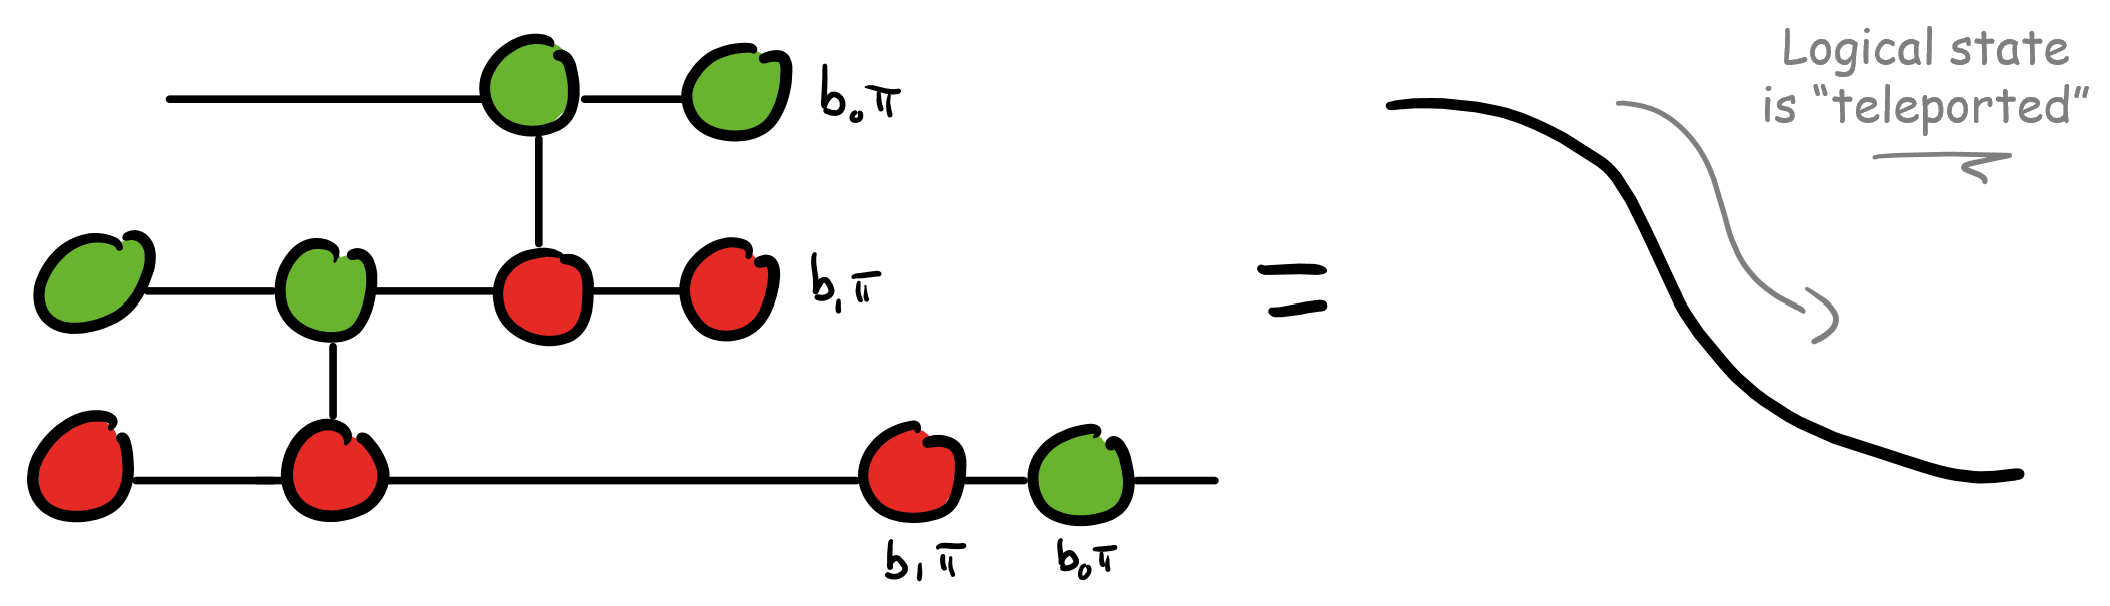
\includegraphics[width=0.45\textwidth]{Sections/pictures/teleportation-diag-reasoning.png}
\end{center}
In the QP approach, the same diagram that describes the protocol simultaneously provides the medium upon which any associated calculations can be performed.
This contrasts with the traditional Hilbert space approach, where different languages are used for calculation (bra-ket notation) and description (quantum circuit notation).
Calculations in the QP framework proceed by applying ``substitution rules'', graphical modifications of diagrams that maintain their meaning, i.e. that result in different diagrams with the same effect (symbolised by the equal sign).
Figure \ref{fig:zx-rules} (p.\pageref{fig:zx-rules}) presents some of the substitution rules for the ZX-calculus used by the examples in this paper. With the addition of only a few more other rules to the ones shown in Fig. \ref{fig:zx-rules}, the set of substitution rules is complete, i.e. suffices to make the ZX-calculus as expressive as the Hilbert space formalism for qubits~\cite{hadzihasanovic2018two} and more generally, for arbitrary finite dimension~\cite{poor2023completeness}.

As a warm-up exercise in diagrammatic substitution, below is the proof that two CNOT gates in sequence cancel each other out, leaving the two qubits---the two wires running left to right---unchanged.
\begin{center}
    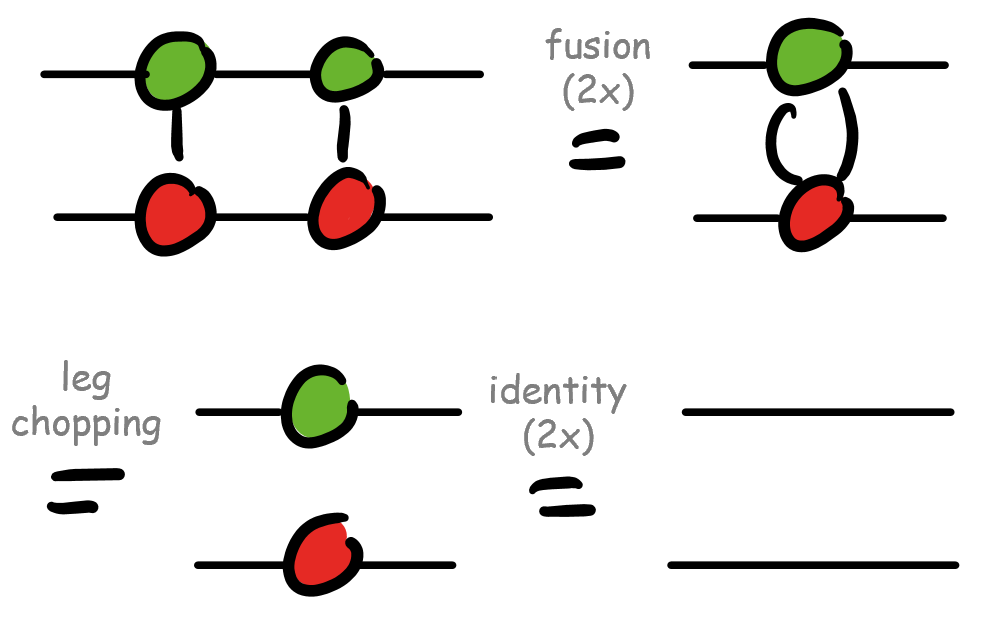
\includegraphics[width=0.3\textwidth]{Sections/pictures/double-cx-two-lines.png}
\end{center}
The proof consists of two steps.
As the first step, we apply the ``fusion'' rule twice (cf. Fig. \ref{fig:zx-rules}, left): once to fuse the two green spiders, once to fuse the two red spiders.
As the second step, we apply the ``leg chopping'' rule (cf. Fig. \ref{fig:zx-rules}, middle top), to remove the pair of legs between the red and green spiders.
The results are two undecorated wires, carrying the two qubits from input to output unaltered.

% As a second warm-up exercise, below is the proof that three alternating CNOT gates have the same effect as swapping two qubits.
% This is an important practical observation in quantum computing, use to compile quantum circuits in architectures---such as superconducting quantum computers---where CNOT gates can only be performed between a small number of qubit pairs.
% \begin{center}
%     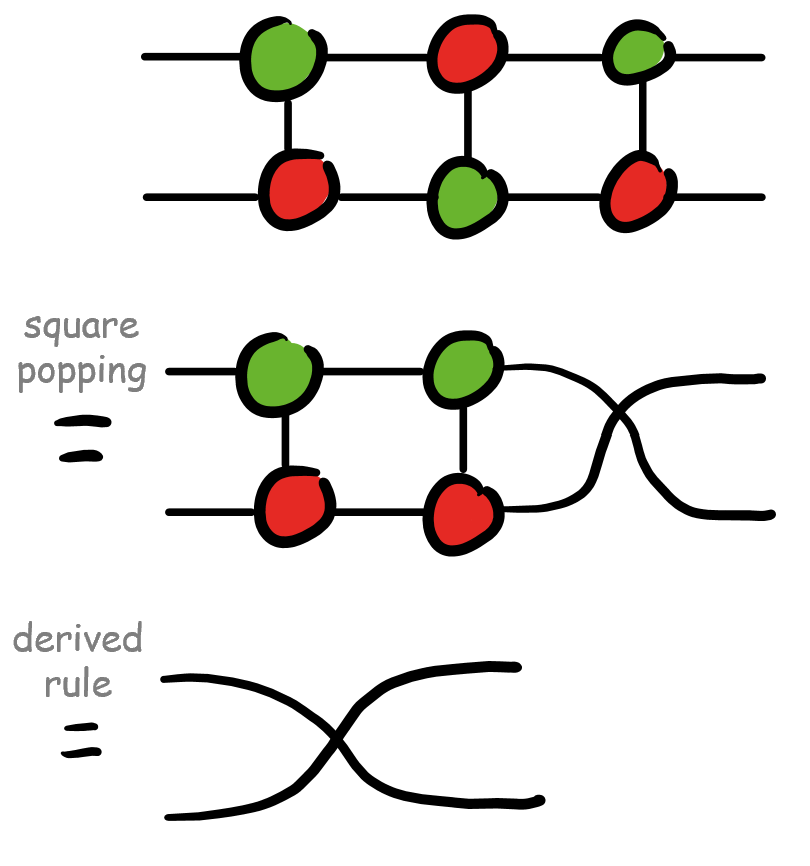
\includegraphics[width=0.25\textwidth]{Sections/pictures/triple-cx-three-lines.png}
% \end{center}
% The proof consists of two steps.
% As the first step, we apply the ``square popping'' rule (cf. Fig. \ref{fig:zx-rules}, middle bottom) to the rightmost two CNOTs, replacing them with a CNOT and a qubit swap.
% As the second step, we apply the equation from the previous exercise as a ``derived rule'', removing the two CNOTs and leaving the desired swap.

Now familiar with the diagrammatic substitution, we can focus on Figure \ref{fig:diagrammatic-reasoning-teleportation-steps} above, presenting the full proof of correctness for the quantum teleportation protocol.

The natively visual character of QP makes it easy to augment diagrams with other kinds of visual information, synergistically enhancing the communication power of all media involved.
For example, below is an explanation of how the fusion rule (cf. Fig. \ref{fig:zx-rules}, left) implements the action of rotation gates on quantum states.
\begin{center}
    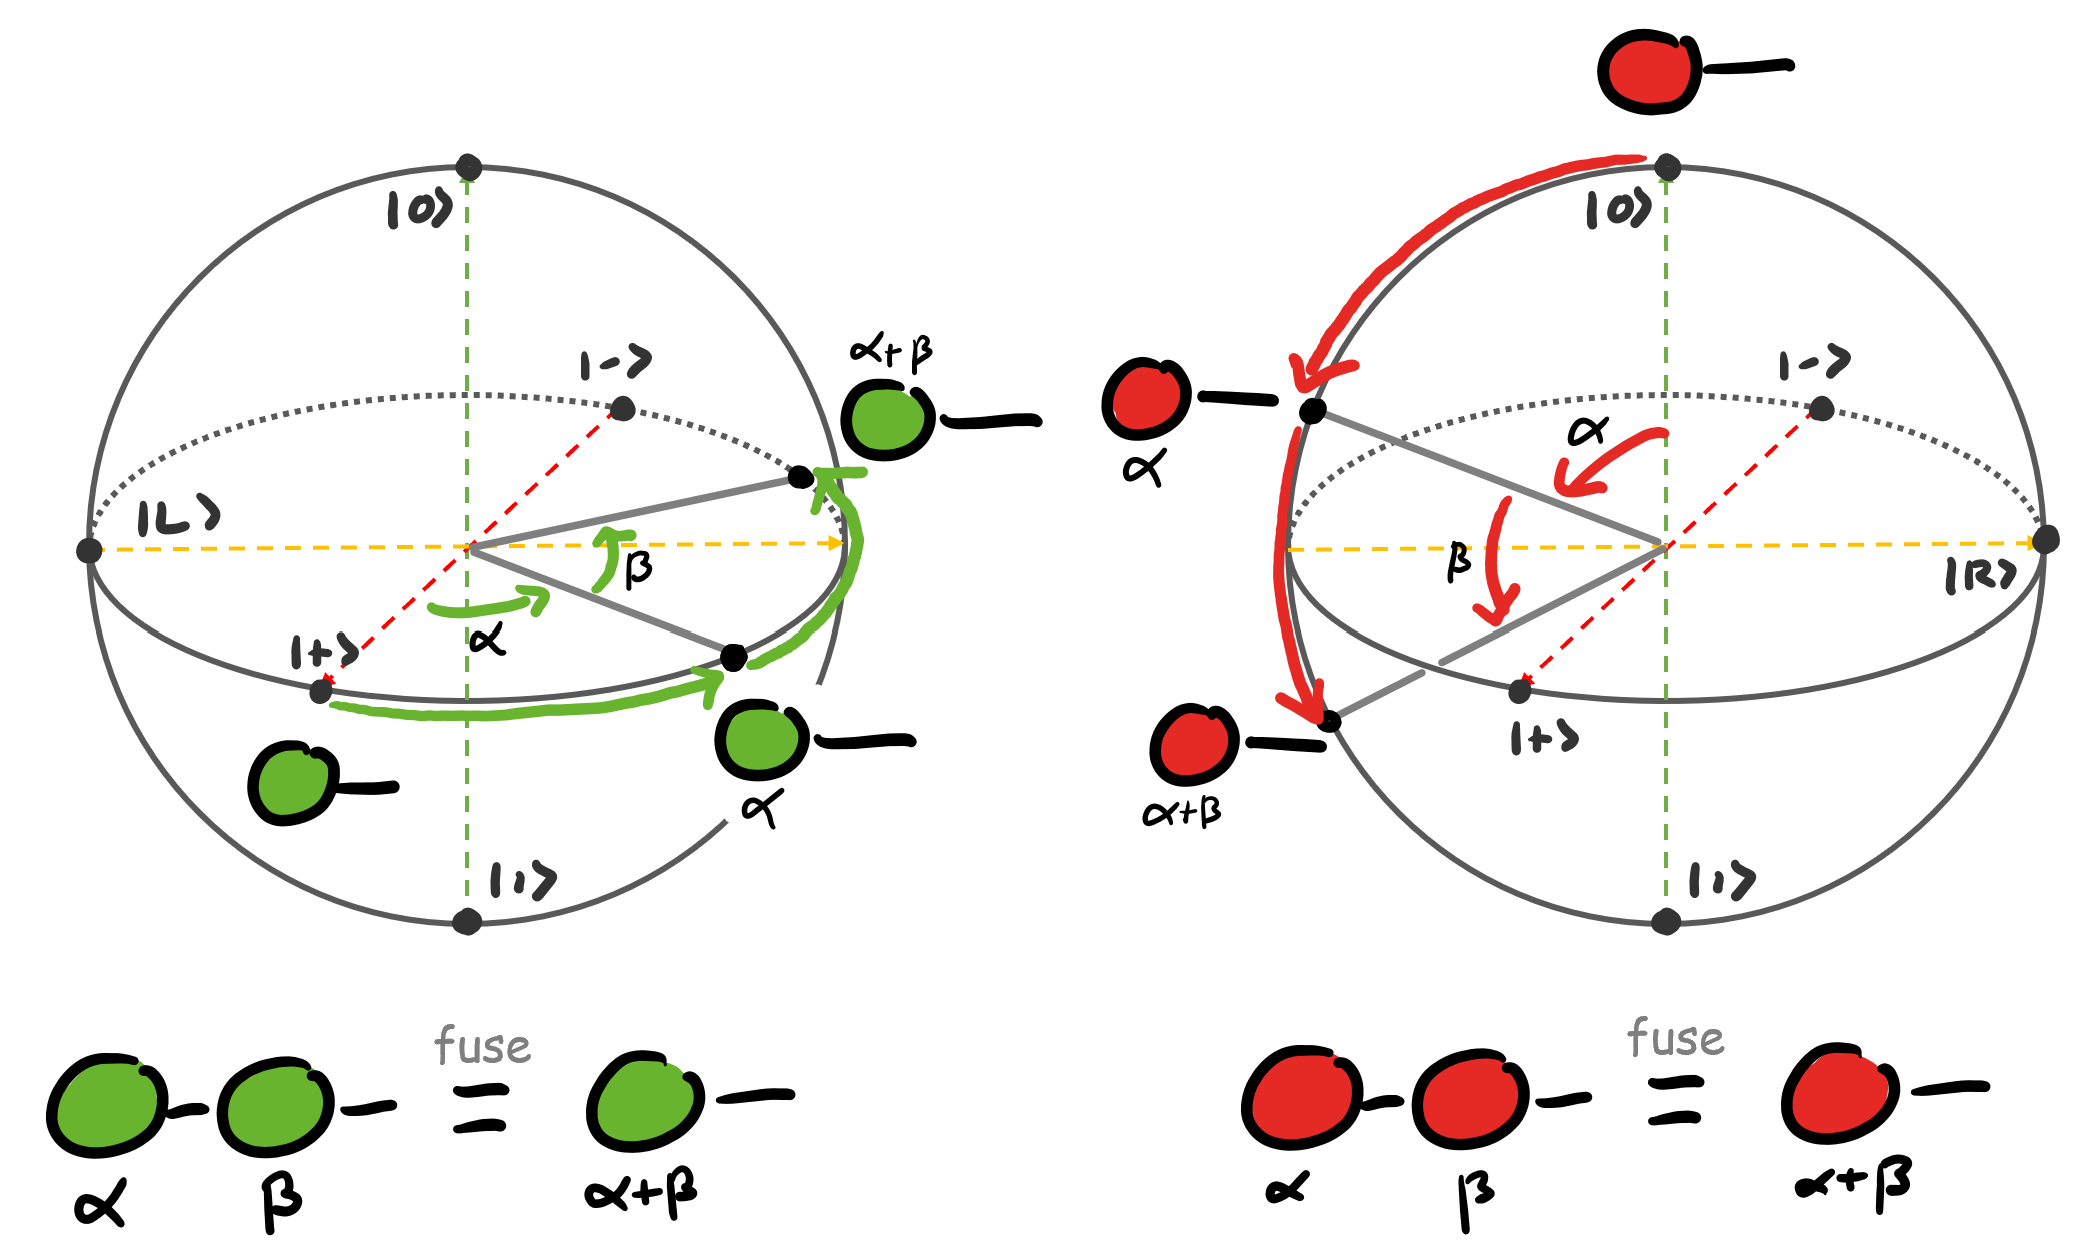
\includegraphics[width=0.5\textwidth]{Sections/pictures/spider-states.png}
\end{center}
The Bloch spheres endow the spiders with additional geometric meaning, locating them on the equator and prime meridian based on their phase.
The fusion rule, on the other hand, enhances the Bloch sphere presentation by adding a dynamical, computational description of the rotation action.

Diagrams are also easily augmented by non-technical conceptual art to convey meaning that exceeds the boundaries of mathematical and physical rigour.
For example, below is a diagrammatic representation of the Bell test, where an entangled state is measured simultaneously by two parties at a large distance apart.
\begin{center}
    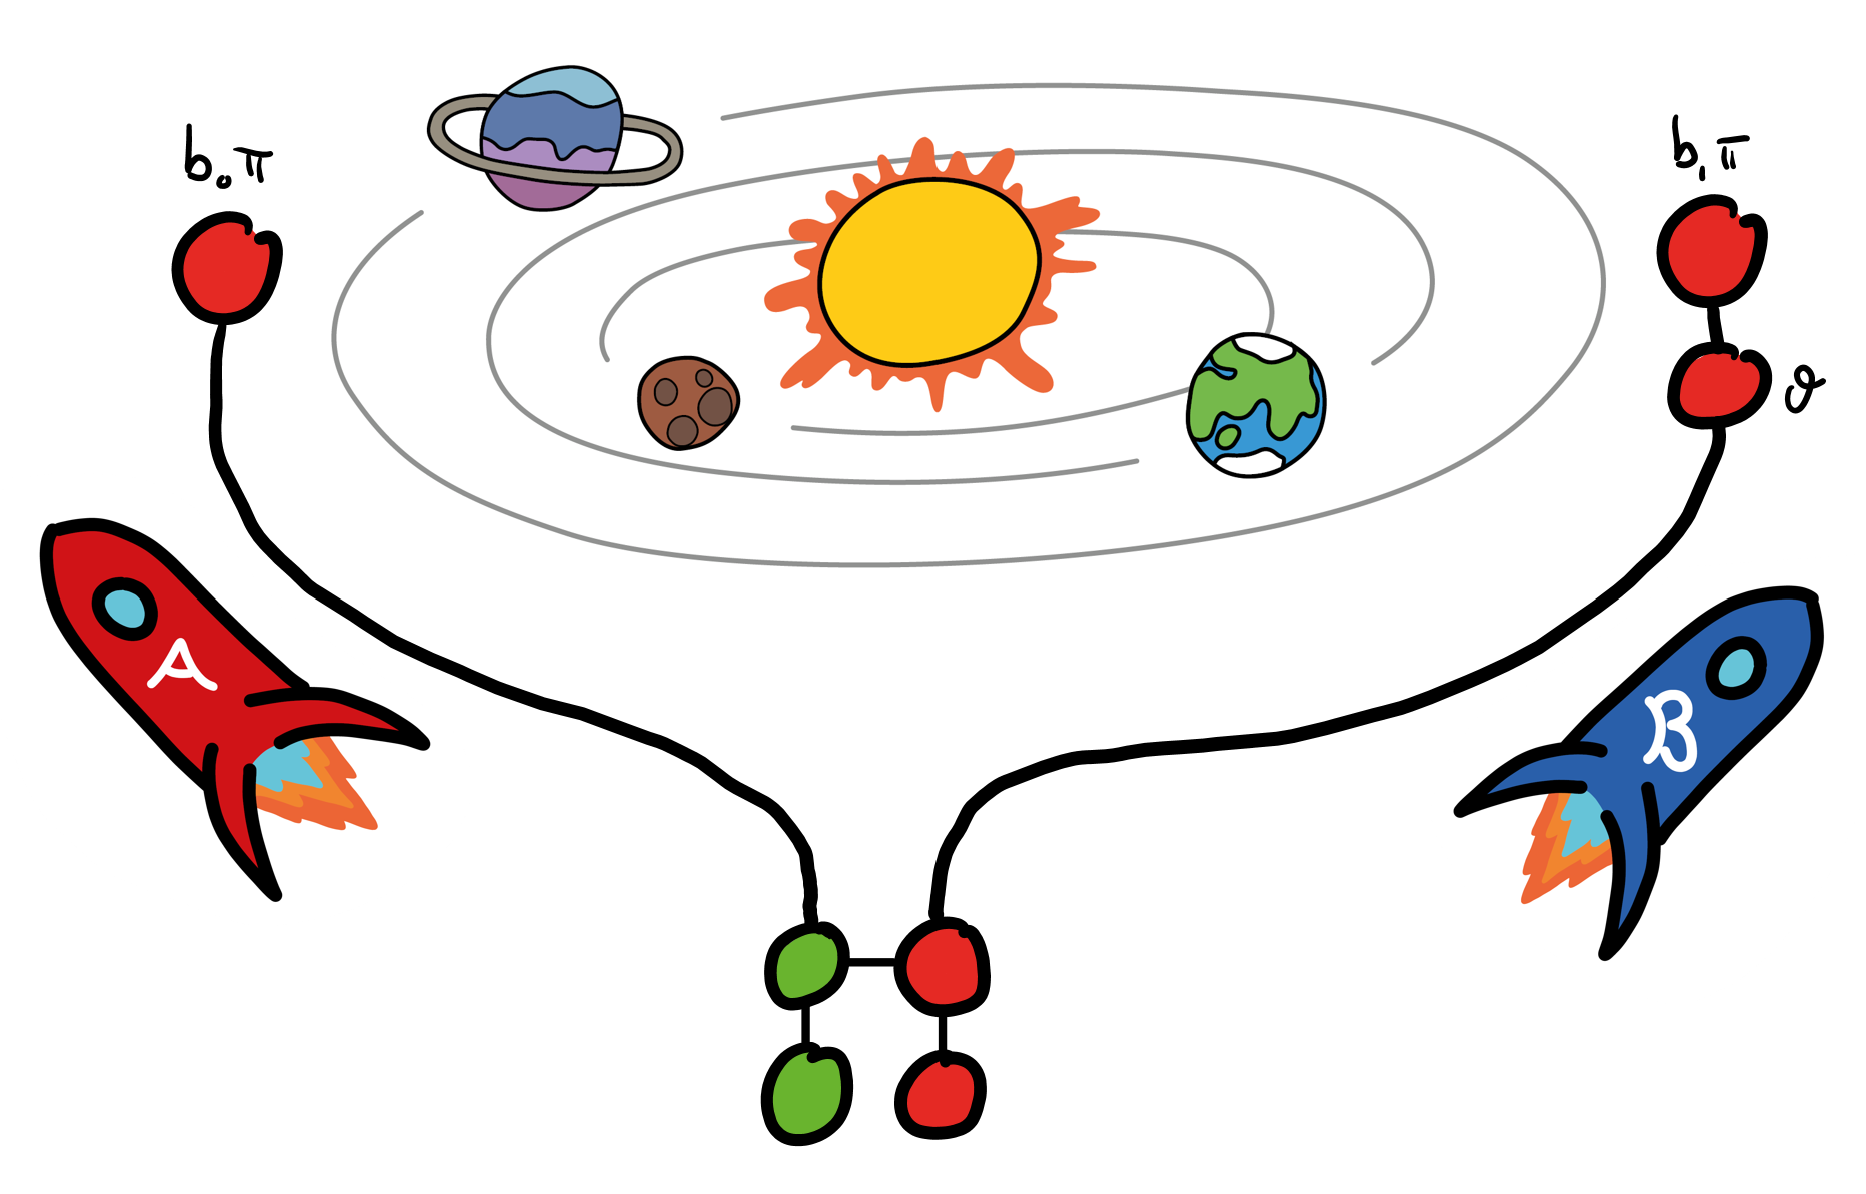
\includegraphics[width=0.4\textwidth]{Sections/pictures/diagrams-mixed-media.png}
\end{center}
The diagram is enriched by a number of artefacts and considerations.
Firstly, the diagram is drawn bottom-to-top\footnote{As opposed to the left-to-right convention, which we have previously adopted to represent the quantum teleportation protocol, matching the directional convention of quantum circuit notation.} to match worldline diagrams from general relativity.
Secondly, drawings of rockets and a solar system are used to indicate that, after becoming entangled, the two qubits are moved very far from each other.
Finally, the two measurements are horizontally aligned to indicate the (approximate) simultaneity of the operations performed by the two parties at a distance.

Finally, the diagrammatic representation itself can reveal hidden spatial structures within quantum algorithms, which may help explain how and why such algorithms work.
For example, below is a diagrammatic representation of the Quantum Approximate Optimisation Algorithm (QAOA), applied to solve the max-cut problem\footnote{An important combinatorial optimisation problem on networks. The max-cut problem is ``NP-complete'', i.e. solutions to this problem translate into solutions for a large class of problems of enormous real-world significance.} on a small network (6 nodes, corresponding to 6 qubits).
The traditional presentation of this algorithm (left below) uses initial states, CNOT gates, Z rotations and measurements, much as the quantum teleportation algorithm previously discussed.
By exploiting the visual flexibility of the QP approach, we repeatedly apply the fusion and square-popping rules (cf. Fig. \ref{fig:zx-rules}) and re-arrange the spider layout until the simplified diagram (right below) is obtained.
\begin{center}
    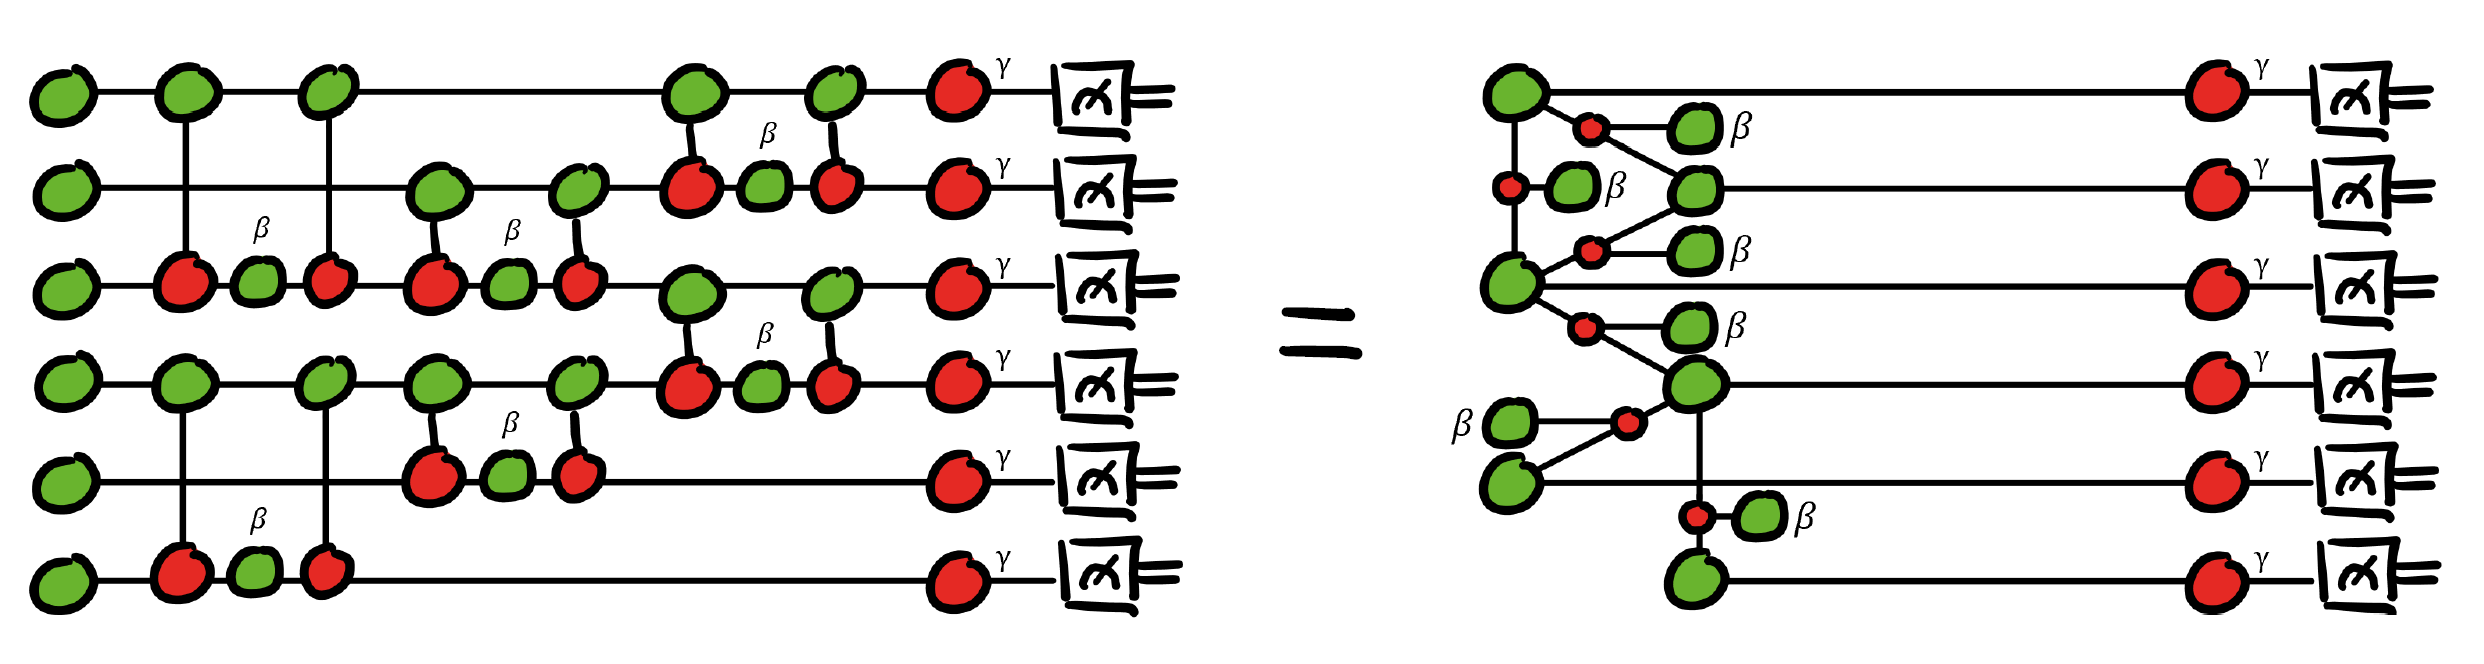
\includegraphics[width=0.48\textwidth]{Sections/pictures/diagrammatic-reasoning-qaoa-eq.png}
\end{center}
The structure of the network (6 nodes connected by 6 edges, drawn in blue, left below) is revealed within the simplified and re-arranged diagram (spiders and wires highlighted blue, right below), exposing the mechanism that ultimately powers QAOA: the ability to entangle quantum systems in a way which matches the constraint pattern of the chosen optimisation problem.
The algorithm parameters---the $\beta$ and $\gamma$ angles below---allow the quality and degree of entanglement to be tuned, exploring the space of solutions in directions determined by the entanglement pattern.
\begin{center}
    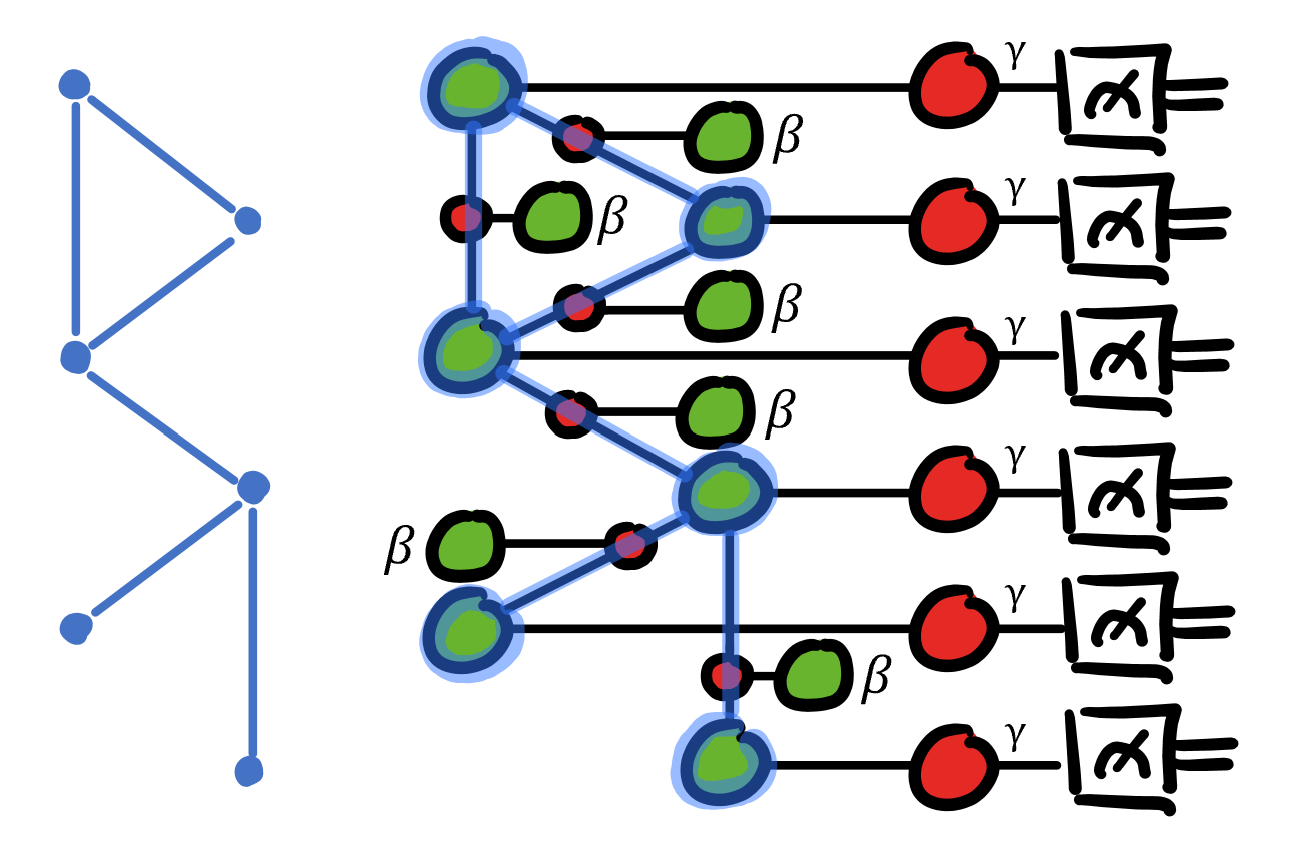
\includegraphics[width=0.34\textwidth]{Sections/pictures/qaoa-circ.png}
\end{center}


% In analogy to the history of classical computer science, the Hilbert space formalism is to low-level assembly code what QP is to high-level programming languages. The Hilbert space formalism may have well been enough to get us through the early days of quantum computer science, but the exponential increase in complexity will soon necessitate higher-level methods, to bring forward applications that would be unimaginable with low-level conceptual tools alone.
